\lab{Applications}{Voronoi Diagrams and Delaunay Triangulations}{Voronoi Diagrams and Delaunay Triangulations}
\label{lab:voronoi}

\objective{Introduce Voronoid Diagrams and Delaunay Triangulations and discuss their applications}

\section*{Voronoi Diagrams}

In this lab we will discuss some applications of Voronoi Diagrams.
In the abstract sense, a Voronoi diagram is a partition of a plane into regions that lie closest to different points.
The easiest way to understand this is to look at some examples.
Figure \ref{voronoi_ex_1} is a voronoi diagram generated from 100 random points with $x$ and $y$ values between 0 and 1.
Notice how each point has a small  cell around it that is made up of the points that lie closest to it.

\begin{figure}
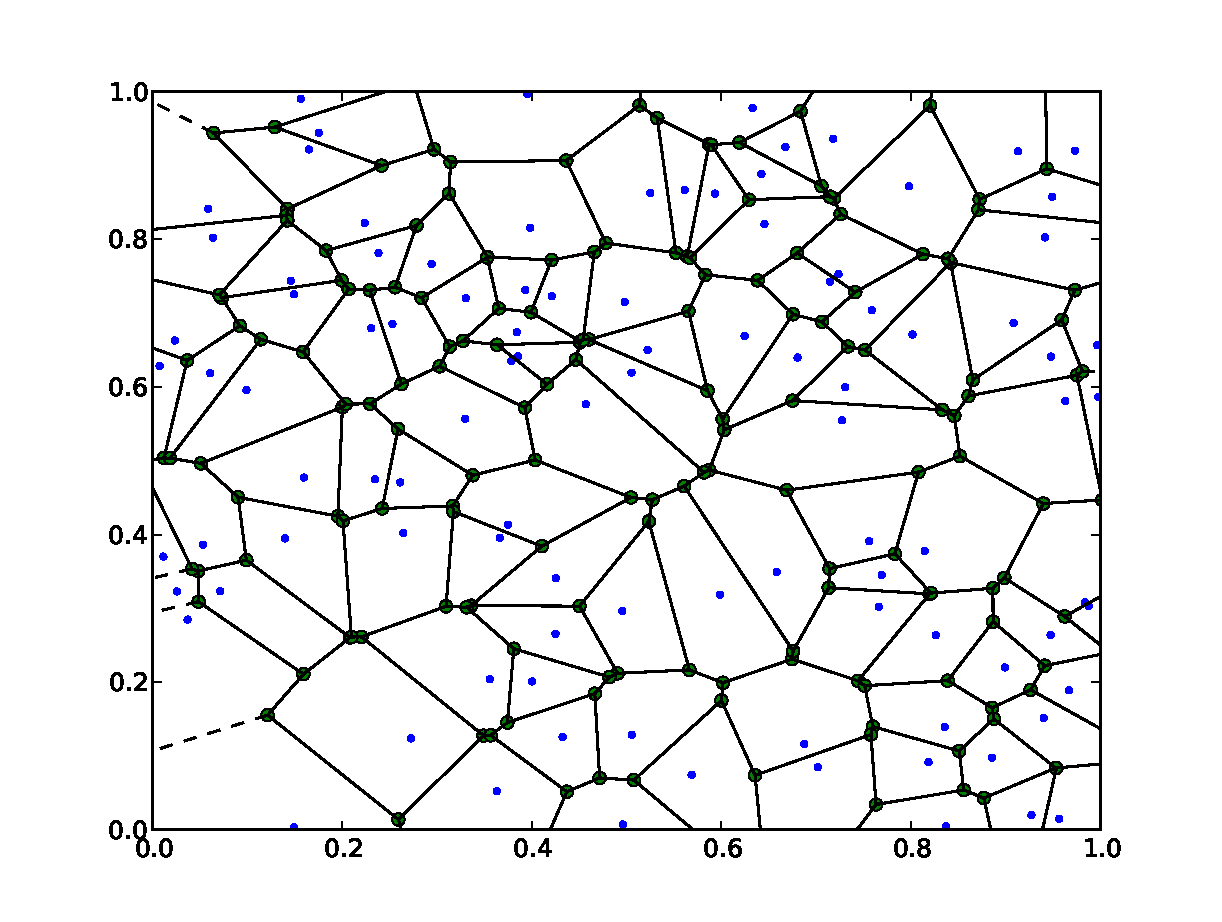
\includegraphics[width=\textwidth]{voronoi_example_1.pdf}
\caption{A Voronoi diagram of the square $[0,1]\times [0,1]$ for 100 randomly generated points.}
\label{voronoi_ex_1}
\end{figure}

One possible way to compute this sort of diagram would be by brute force, for example:
\begin{lstlisting}
import numpy as np
from numpy.random import rand
from matplotlib imort pyplot as plt
num = 10
res = 201
pts = rand(num, 2)
X = np.linspace(0, 1, res)
Y = X.copy()
X, Y = np.meshgrid(X, Y)
Z = np.empty_like(X)
indices = np.zeros_like(X)
for i in xrange(res):
    for j in xrange(res):
        #note: we don't need to do the sqare root
        #since we really just need to compare the distances
        mn = (X[i,j] - pts[0,0])**2 + (Y[i,j] - pts[0,1])**2
        for k in xrange(1,num):
            dist = (X[i,j] - pts[k,0])**2 + (Y[i,j] - pts[k,1])**2
            if dist < mn:
                indices[i,j] = k
                mn = dist
plt.pcolormesh(X,Y,indices)
plt.scatter(pts[:,0],pts[:,1])
plt.xlim((0,1))
plt.ylim((0,1))
plt.show()
\end{lstlisting}
This algorithm is good because it can work regardless of the metric space we are using, but it is terribly slow.
Figure \ref{voronoi_1norm} shows a similar diagram using the 1-norm and figure \ref{voronoi_supnorm} shows a diagram generated using the supremum norm.
It is linear in the number of points added and linear in the number of pixels used to represent the diagram.
This can be a terrible limitation, but if you are not working in a well behaved metric space, this may be the simplest approach.
\begin{figure}
\begin{minipage}[b]{0.45\linewidth}
\centering
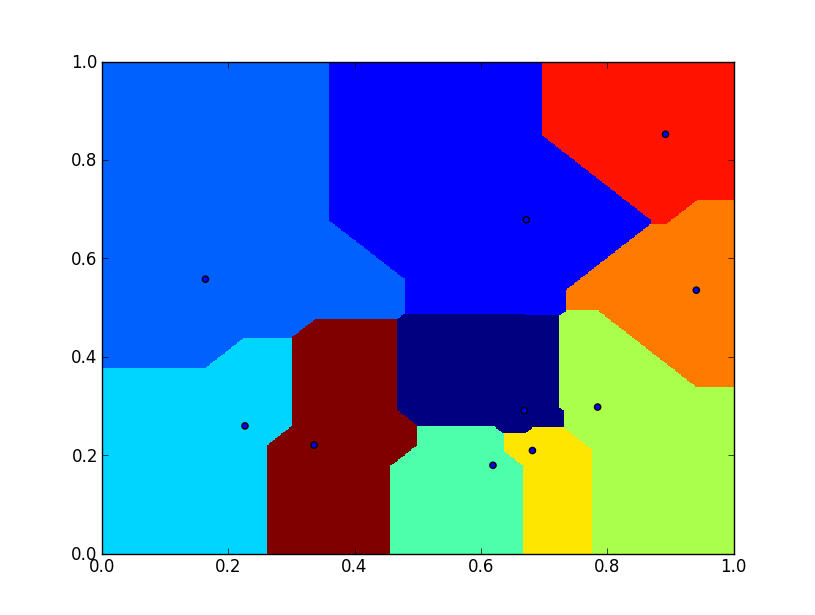
\includegraphics[width=\textwidth]{voronoi_1norm.png}
\caption{Voronoi diagram in the 1-norm}
\label{voronoi_1norm}
\end{minipage}
\hspace{0.5cm}
\begin{minipage}[b]{0.45\linewidth}
\centering
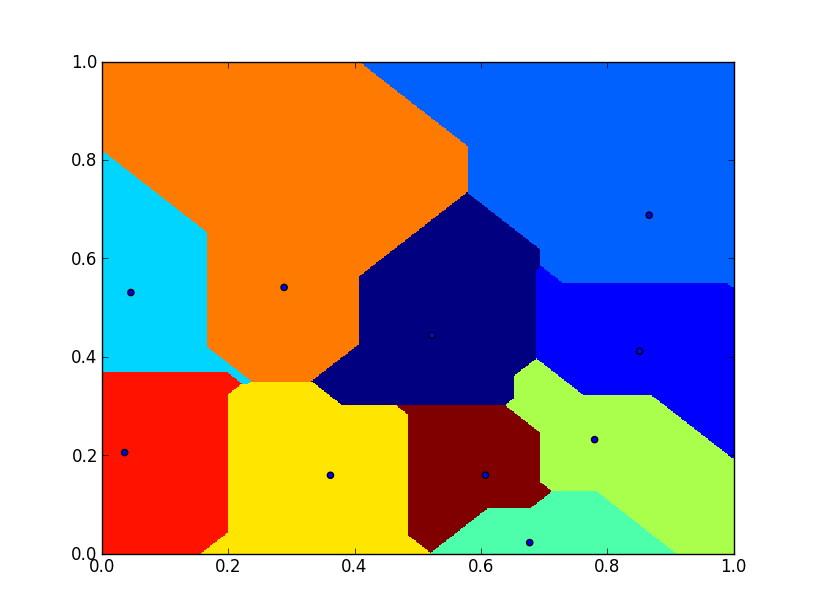
\includegraphics[width=\textwidth]{voronoi_supnorm.png}
\caption{Voronoi diagram in the supremum norm}
\label{voronoi_supnorm}
\end{minipage}
\end{figure}

It is also possible to make voronoi diagrams based off of shapes and lines as well as points. 

There are several data structures used in the field of computational geometry that can store the exact edges of diagrams like this.
We would prefer to not have to worry about sampling the domain in this way.
There are a variety of algorithms that can compute Voronoi diagrams in $\mathcal{O}\left( n \log\left(n\right)\right)$ time (where $n$ is the number of points).
Fortune's algorithm is a linesweep algorithm that can do this.

The Qhull library is commonly used to compute voronoi diagrams, and delaunay triangulations.
SciPy includes a wrapper of the Qhull library in the \li{scipy.spatial} module.
It currently only supports 2 dimensional voronoi diagrams under the Euclidean norm.
It allows you to generate a voronoi diagram from a set of points, add points to a voronoi diagram, find the nearest point to any given point, and plot a voronoi diagram.

A plot similar to the one we just generated can be made using SciPy like this:
\begin{lstlisting}
import numpy as np
from numpy.random import rand
import scipy.spatial as st
from matplotlib import pyplot as plt
G = rand(100,2)
G = st.Voronoi(G)
st.voronoi_plot_2d(G)
plt.xlim((0, 1))
plt.ylim((0, 1))
plt.show()
\end{lstlisting}
Notice how much clearer the plot is and how much faster it is generated.
Try running the last bit of code for 1000 points.
Though this is a little slower than it was for 10 points, this is a graph that would not display well if we had been using the brute force method.

Table \ref{voronoi_attributes} shows the different attributes of the \li{Voronoi} object.
For more details, see \url{http://docs.scipy.org/doc/scipy-dev/reference/spatial.html}
\begin{table}[h!]
\begin{center}
	\begin{tabular}{|l|p{12cm}|}
    \hline

    \li{points} & coordinates of input points (centers of cells)\\

    \li{vertices} & vertices of graph\\

    \li{ridge_points} & indices of the input points between which each ridge on the diagram lies\\

    \li{ridge_vertices} & indices of the vertices at the end of each ridge\\

    \li{regions} & indices of the vertices corresponding to each voronoi cell\\

    \li{point_region} & indices of the regions corresponding to each input point\\

    \hline

    \end{tabular}
\end{center}
\caption{Various summarizing functions}
\label{voronoi_attributes}
\end{table}

Unfortunately, the \li{Voronoi} objects do not allow us to find out, given the coordinates of a new point, which of our original input points lies the closest to it.
To do something like that we would need to use a different algorithm or data structure.
One possible way of solving such a problem is to us a KD tree.
KD trees will be discussed in further detail in Volume II.
Scipy includes built in KD trees in both Python and C.
The version in C is generally faster.
You can make a KD tree like this
\begin{lstlisting}
import numpy as np
from numpy.random import rand
import scipy.spatial as st
A = rand(1000,2)
kd = st.cKDTree(A)
\end{lstlisting}
In this case we used the \li{cKDTree} object.
That is a KDTree implemented in C.
\li{KDTree} is a Python-based version that is also included in scipy.

\section*{Applications of Voronoi Diagrams}

Though the computation of a Voronoi Diagram does not provide a quick way to run nearest neighbor queries, there are still several applications for Voronoi Diagrams.
The first, and probably most obvious, is the representation of data.
If you want to look for visual patterns in data, a Voronoi Diagram can be very useful.
One historically significant example was the containment of the London Cholera outbreak of 1854.
The English Mathematician John Snow plotted where the cholera outbreaks had all happened and after some consideration, noticed that they were all relatively close to a certain water pump in that portion of the city.
Upon noticing this, he plotted the voronoi cell of that particular water pump and proposed that the cholera outbreak was linked to contaminated water.
He recommended that the pump handle be removed so that people would have to use other pumps in the city.
Once the contaminated pump was shut down, the cholera outbreak was stopped.

Voronoi diagrams can also be used to solve problems involving the points furthest from those already on the graph.
Examples include determining where to drill next when searching for oil, or where to put a new branch of a major company.

\begin{problem}
For Problems \ref{FurthestPoints} and \ref{AverageRainfall} it will be useful to be able to restrict a voronoi diagram to a given square region.
Write a function that, given a Voronoi Diagram and the constraints for a rectangular region, returns modified versions of the \li{vertices}, \li{regions}, and \li{point_region} representing the cells formed by the intersection of the Voronoi diagram with the rectangle.

%% give more detail here because this could be very hard without help.
%% maybe we should give this one to them outright.

\end{problem}

\begin{problem}
\label{FurthestPoints}
Write a function that, given a list of points and a rectangular region of the plain and an integer $n$, finds the $n$ points in the region that lie farthest from all the points already given.
\end{problem}

Another possible application is navegation through a field of obstacles.

\begin{problem}
Given a list of points, form the adjacency matrix corresponding to the connections between each node of the Voronoi diagram.
Use your solution to Lab \ref{lab:MarkovGraph} Problem \ref{maze_prob} to find a path from any given node to any other node.

Note: if you have worked the lab on Djikstra's Algorithm in Volume 2, you may use your solution to that lab and give the graph weights corresponding to the distance between nodes instead.
\end{problem}

Another possible application of voronoi diagrams is in the estimation of total rainfall, size of ore deposits, or other similar problems.
One simple way to do this is to take a weighted average of all known measurements where each measurement is given the weight corresponding to the size of its voronoi cell.

\begin{problem}
\label{AverageRainfall}
Write a function that, given a square region and measurement values at different nodes, computes the weighted average of the measurements over the region.
Weight each measurement according to the area of the voronoi cell of each node.

Hint: You can find the area of each voroni cell by considering the triangles formed between its vertices and its center point. One way to compute the area of a triangle given the coordinates of its vertices is $A = \sqrt{s\left(s-a\right) \left(s-b\right) \left(s-c\right)}$ where $s = \frac{a+b+c}{2}$ and $a$, $b$, and $c$ are the vertices of the triangle.
This is known as Herron's Formula.
\end{problem}

\section*{Delaunay Triangulation}

A concept related to Voronoi diagrams is that of the Delaunay Triangulation.
Delaunay Triangulations also have a wide variety of applications.
One such application is the automatic division of a region into triangles for use in finite element analysis for the numerical solution of partial differential equations.
In general, the delaunay triangulation divides the smallest convex region containing all the given points (the convex hull) into triangles that obey certain rules.

You can make a Delaunay Triangulation from a list of points and plot it like this:
\begin{lstlisting}
A = rand(100, 2)
D = st.Delaunay(A)
plt.triplot(A[:,0] ,A[:,1], D.simplices)
plt.show()
\end{lstlisting}

\begin{problem}
Use a Delaunay triangulation to write a function that breaks up the unit square into right triangles.
Have the only argument to your function be the number of nodes you want along each edge of the square.
Plot your results.
\end{problem}

%other possible applications:
%Use Delaunay Triangulation to tesselate a 3d surface.
%Use tesselation to rerun ore/rainfall problem and compare results.